\section{Application Implementation}
This section will describe the implementation of the study application, mostly regarding how data was collected, how features were computed as well as how the data was sent to a Firebase instance. The study app used the package while it was in an earlier iteration. In this iteration, almost none of the logic related to storing and loading data was part of the package, and as such all of this had to be written in the application instead. This section will provide source code examples of how the application should be implemented with the new API since the old version is deprecated. Largely, the data flow of the study app has not changed but the concrete implementation has, in the sense that much fewer lines of code are needed.

\subsection{Architecture Overview}
To provide a high-level overview of the different components which make up the study application, a component diagram displayed in Figure \ref{fig:app-component-diagram}. The MobilityStudy component in blue is the component responsible for managing the application state but does not do much outside of this since the application state management required is minimal. Had it been a more complex application with many different screens and a state which had to be maintained across these screens (for example a shopping cart in a shopping app) then more logic would lie inside the MobilityStudy component. Instead, the Main Screen is spawned from the MobilityStudy component which in turn creates an AppProcessor instance. The AppProcessor instance is responsible for a multitude of tasks, such as asking for permissions, collection location data, and computing features. Storing and loading from the disk is done through the FileManager component which includes location data, Stops, Moves, MobilityContexts, and diary answers. This component is also responsible for uploading the stored data to Firebase.

\begin{figure}
    \centering
    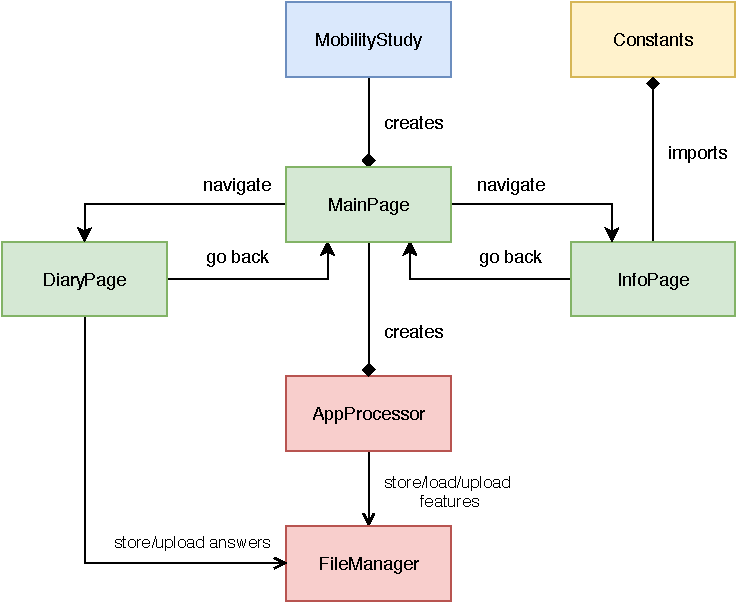
\includegraphics[width=0.7\textwidth]{images/diagrams/app-diagram.pdf}
    \caption{Component diagram for the study application displaying the different building blocks and the interactions between them}
    \label{fig:app-component-diagram}
\end{figure}

\subsection{Custom Location Plugin}
For collecting Location Samples, a custom version of the \textit{Geolocator}\footnote{\url{https://pub.dev/packages/geolocator}} plugin was developed for the purpose of this package to achieve reliable background location streaming. The current implementation of \textit{Geolocator} was missing a flag in the \textit{Objective-C} implementation for iOS, which allows the app to continue streaming location data while the app is minimized. The flag for background updates has to be set for an instance of a Location Manager which is the access to the Location API:

\begin{minted}{dart}
    _locationManager.allowsBackgroundLocationUpdates = YES;
\end{minted}

If this flag is not set to 'YES' (i.e. True), the location stream will die shortly after the application is minimized. It is important to note that this plugin is not part of the Mobility Features Package, but is likely needed to make use of the package. A Github issue was created\footnote{\url{https://github.com/Baseflow/flutter-geolocator/issues/390}} and the features were merged to a development branch for the GeoLocator plugin. The functionality is however not public as of yet, and the custom plugin was, therefore, necessary to use when developing the application. 

\subsection{Collecting Location Samples}
The custom Geolocator plugin was used to set up a stream of location data. The DTO of the plugin called Position, and contains latitude, longitude, and timestamp, in addition to other GPS information. The stream is set up with a subscription using a call-back method that is invoked every time a Position object is generated by the stream. 

\begin{minted}{dart}
await _geoLocator.isLocationServiceEnabled().then((response) {
  if (response) {
    streamingLocation = true;
    _subscription = _geoLocator.getPositionStream(options).listen(_onData);
  } else {
    print('Location service not enabled');
  }
});
\end{minted}

This call-back method is the \verb|_onData| method which is responsible for saving the collected data. It does so by first converting the Position DTO object into a LocationSample DTO object, and then adding it to a buffer. This buffer is implemented a List of LocationSamples and when the number of samples in this buffer exceeds 100, the content of the buffer will be stored to disk via the \verb|MobilitySerializer|. Afterward, the buffer is emptied, and the process starts anew. 

\begin{figure}
    \centering
    \begin{minted}{dart}
      void _onData(Position x) async {
        GeoPosition gp = GeoPosition(x.latitude, x.longitude);
        LocationSample sample = LocationSample(gp, x.timestamp);
        _buffer.add(sample);

        if (_buffer.length >= BUFFER_SIZE) {
          /// Save buffer locally, empty it,  then upload data
          await _sampleSerializer.save(_buffer);
          _buffer = [];
          await FileManager().uploadSamples(uuid);
    
          /// If enough data has been collected, evaluate features
          numberOfBuffers++;
          if (numberOfBuffers >= 5) {
            numberOfBuffers = 0;
    
            /// Offload computation to background, do not await
            _computeFeaturesAsync();
          }
        }
      }
    \end{minted}
    \caption{The \textit{\_onData} method responsible for handling incoming Location DTOs}
    \label{fig:ondata-method}
\end{figure}


\subsection{Firebase Services}
Firebase file storage was used to host all the data generated by the study application. Another possibility was to use a Firebase Realtime Database however given that the application already used files for storing data, it seemed most natural to continue using a file-based system. File storage hosted on a centralized server made it easy to oversee the study and check in on users to see if they remembered to provide answers and track their location. \\

Additionally, the Firebase Cloud Messaging (FCM) service was set up such that push notifications could be delivered to the participants' phones via the application, to remind them to fill out the diary. Push notifications are another alternative to local notifications, the latter of which is scheduled using alarm-based triggers. Push notifications are a great tool as a developer since notifications are sent out from a centralized server and can be edited at any time without access to the physical phones. In was sometimes useful to send out notifications to specific users if they forgot to fill out many days in a row.

\subsection{Computing Features and Async Calls }
Every time the buffer has been 'spilled' to the disk 5 times, features are computed. This was done simply to ensure features were computed regularly in real-time (i.e. with an incomplete dataset) during the study, as is a completely arbitrary trigger. In addition, whenever the user navigates to the diary page, features are computed such that they are generated close to answers being given. One concept not discussed much so far is the need for asynchronous computation and the use of multi-threading. Flutter applications support multi-threading, which means the main thread runs the user interface, and background threads can be spawned in order to perform heavy computation which would otherwise 'clog' the main thread, which means the user will experience a frozen UI. In the study app, there was no real user interface so to speak, but in a real-world application, there will be a user interface that cannot be allowed to freeze due to the feature calculation. In Flutter threads are referred to as Isolates which communicate using a \textit{SendPort} and a \textit{ReceivePort}. These two objects can be used to transfer other objects between threads, such that the main thread can request a background thread to calculate the features, and the background thread will then send back a \textit{MobilityContext} object once finished. 

\begin{minted}{dart}
Future<MobilityContext> _computeFeaturesAsync() async {
  ReceivePort receivePort = ReceivePort();
  await Isolate.spawn(_asyncComputation, receivePort.sendPort);
  SendPort sendPort = await receivePort.first;

  MobilityContext mobilityContext = await _relay(sendPort);
  return mobilityContext;
}
\end{minted}

The \verb|_relay| method works as an interface between the \verb|_computeFeaturesAsync| method which runs on the UI thread and the static method \verb|_asyncComputation| which runs on the background thread and simply relays messages between the two threads.

\begin{minted}{dart}
Future _relay(SendPort sendPort) {
  ReceivePort receivePort = ReceivePort();
  sendPort.send([receivePort.sendPort]);
  return receivePort.first;
}
\end{minted}

Lastly, the \verb|_asyncComputation| method is static which is due to the computation being done in a separate thread than the main thread. If the objects contained within the \textit{AppProcessor} instance (i.e. in the main thread) were to change their state while computation was ongoing in the background thread, then the resulting computation would produce an outdated result. The \textit{ContextGenerator} is also a static class without a mutable state and can, therefore, be used to compute the Mobility Context without the need for mutable state anywhere in the chain, once the message reaches the background thread.

\begin{minted}{dart}
static void _asyncComputation(SendPort sendPort) async {
  ReceivePort receivePort = ReceivePort();
  sendPort.send(receivePort.sendPort);
  List args = await receivePort.first;
  SendPort replyPort = args[0];

  MobilityContext context =
      await ContextGenerator.generate(usePriorContexts: true);

  replyPort.send(context);
}
\end{minted}

